\section{Panoramic image}

\begin{frame}{\secname}
    Panoramic image reconstruction uses the techniques explain before.
    \begin{figure}
        \centering
        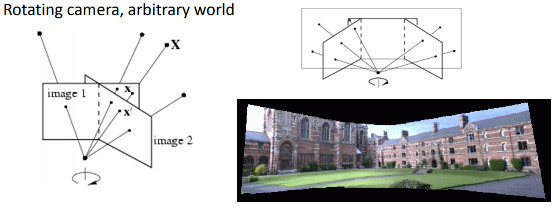
\includegraphics[width=0.8\textwidth]{img/homography_transformation_example3}
        \caption{Panoramic image reconstruction \cite{noauthor_opencv_nodate}}
    \end{figure}
\end{frame}

\begin{frame}{\secname}
    The key points have to be automatically calculated.
    \begin{figure}
        \centering
        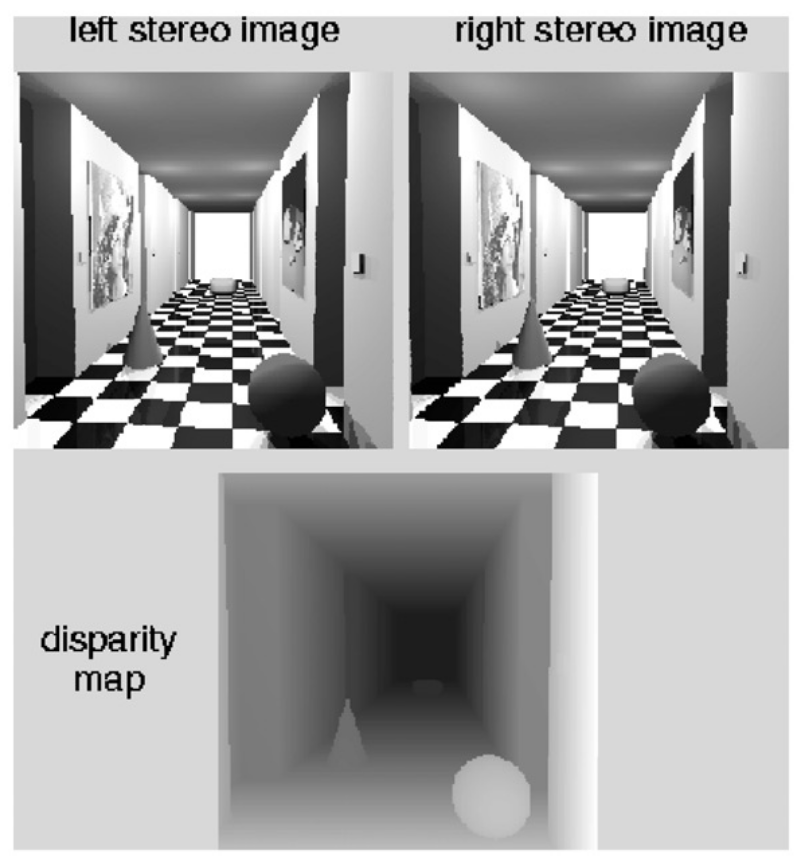
\includegraphics[width=0.5\textheight]{img/pano_make}
        \caption{Stereo images and related disparity map \cite{gledhill_panoramic_2003}}
    \end{figure}
\end{frame}

\begin{frame}{\secname}
    We can use techniques explain during the lessons (Key point feature extraction), such as SIFT, FAST, etc.
    \begin{figure}
        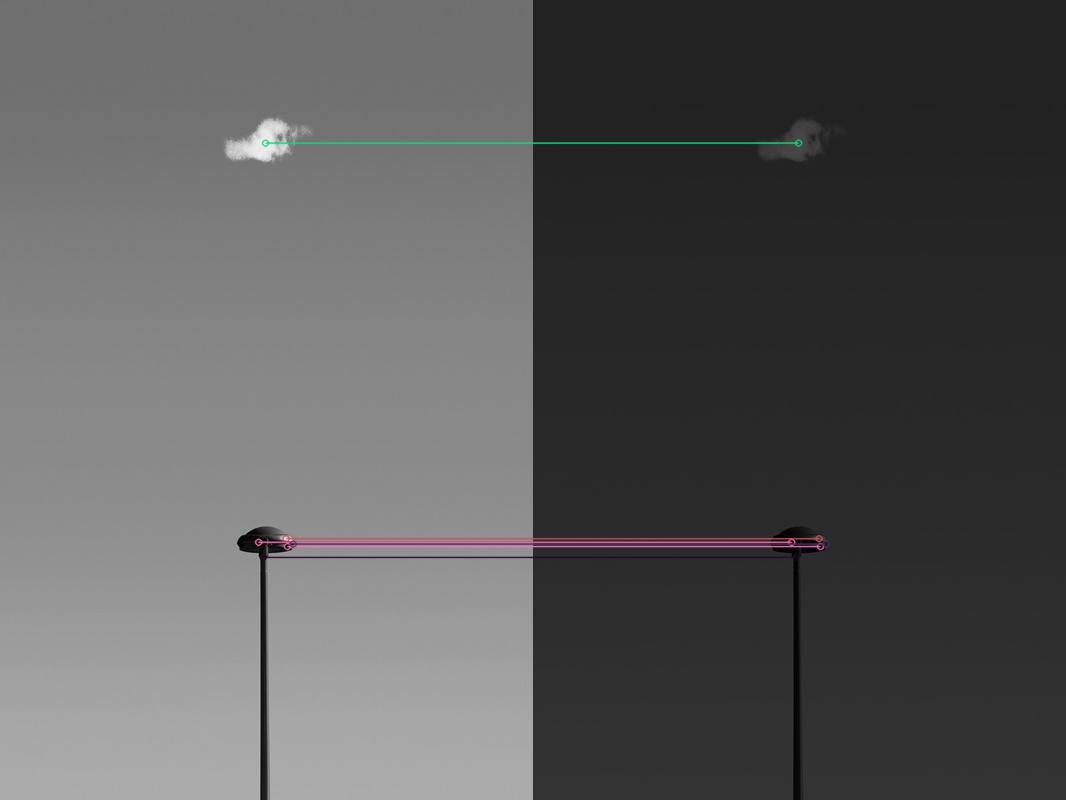
\includegraphics[width=0.5\textwidth]{../doc/sift_algorithm/img/final.png}
        \caption{Key points from practical exercise}
    \end{figure}
\end{frame}

\begin{frame}{\secname}
    If the key points are good enough selected, the results could be quite accurate.
    \begin{figure}
        \centering
        \subfloat[Original images before the mosaic \cite{gledhill_panoramic_2003}]{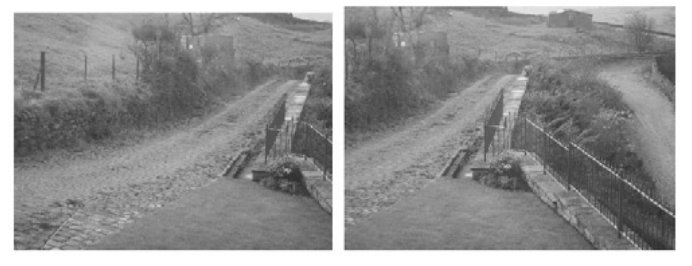
\includegraphics[width=0.5\textwidth]{img/pano_both.png}} \\
        \subfloat[Two images stitched together \cite{gledhill_panoramic_2003}]{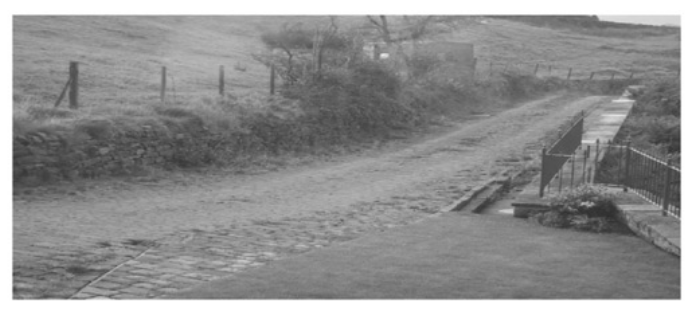
\includegraphics[width=0.5\textwidth]{img/pano_join.png}}
    \end{figure}
\end{frame}

\begin{frame}{\secname}
    This technique can also be used in the reconstruction of non-planar images. \cite{yong_panoramic_2019}
    \begin{figure}
        \centering
        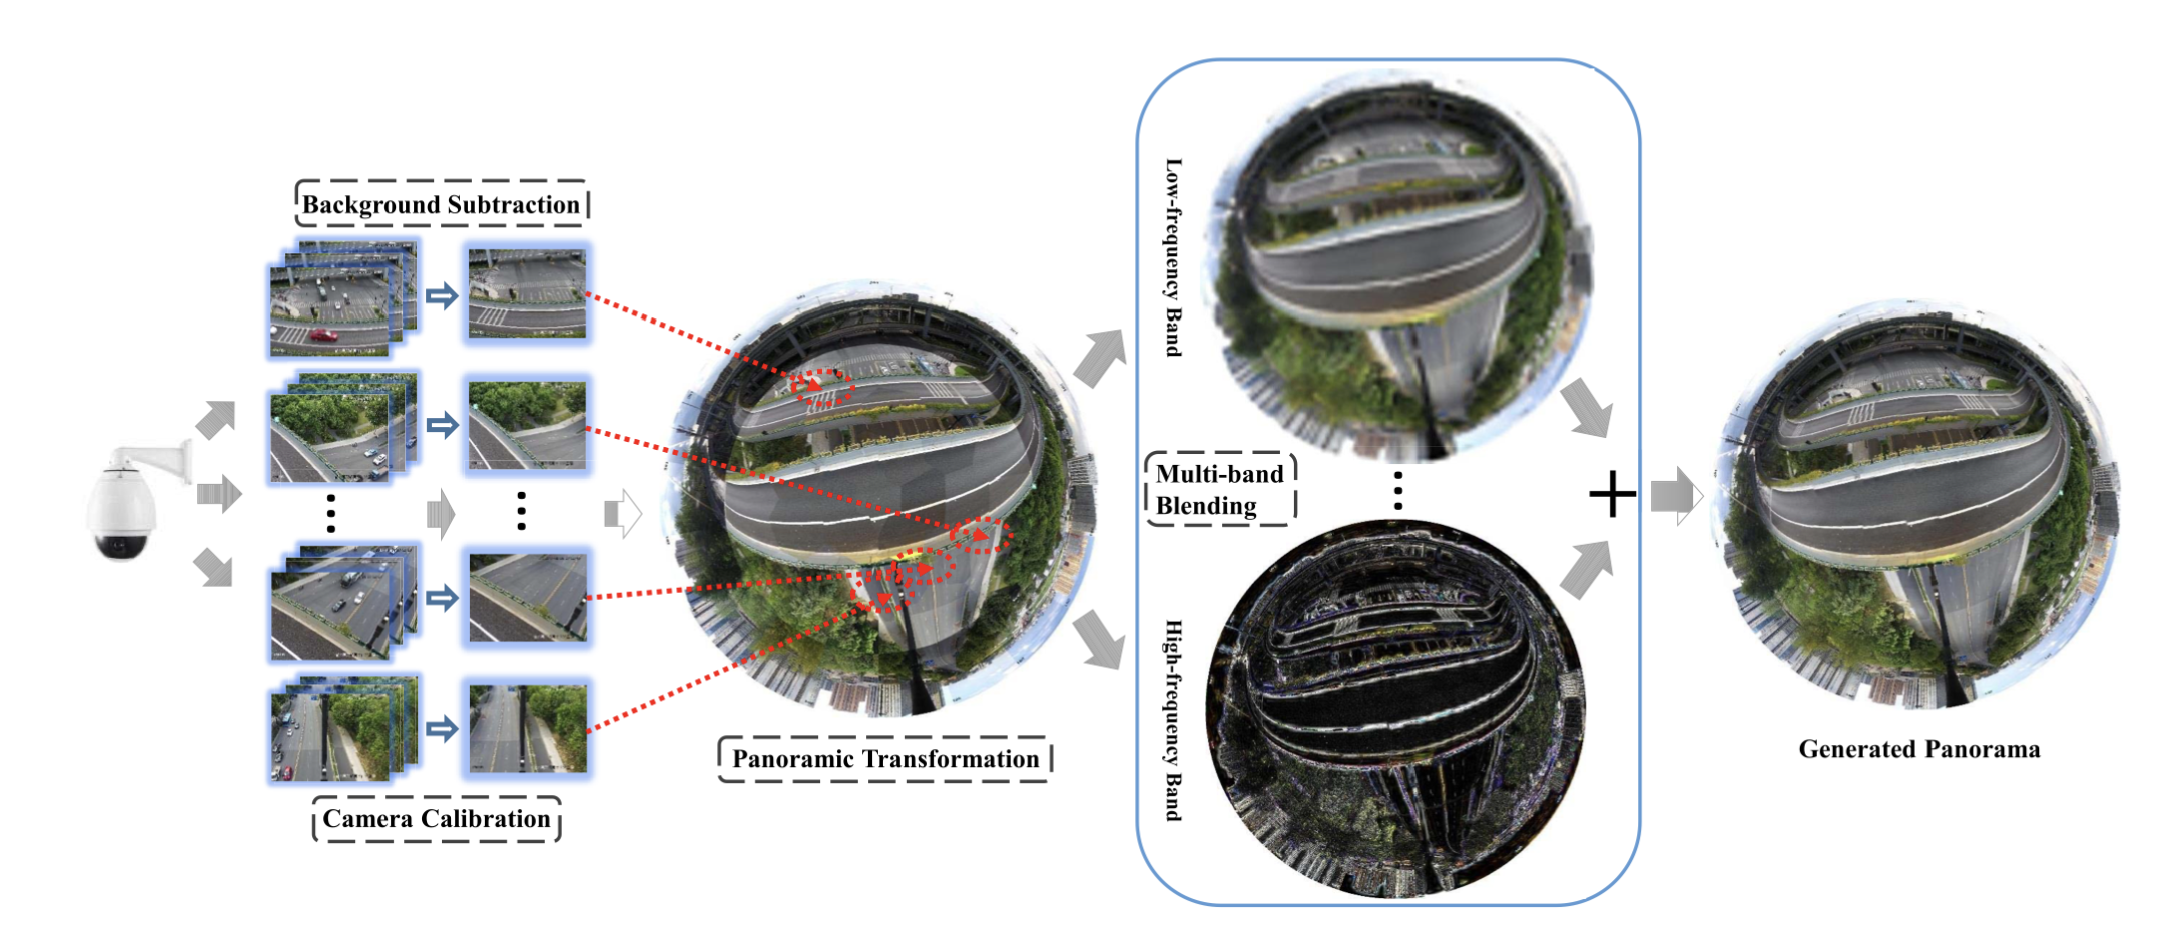
\includegraphics[width=\textwidth]{img/pano_esphere}
    \end{figure}
\end{frame}

\begin{frame}{\secname}
    Another example with a 360º image. \cite{duan_panoramic_2020}
    \begin{figure}
        \centering
        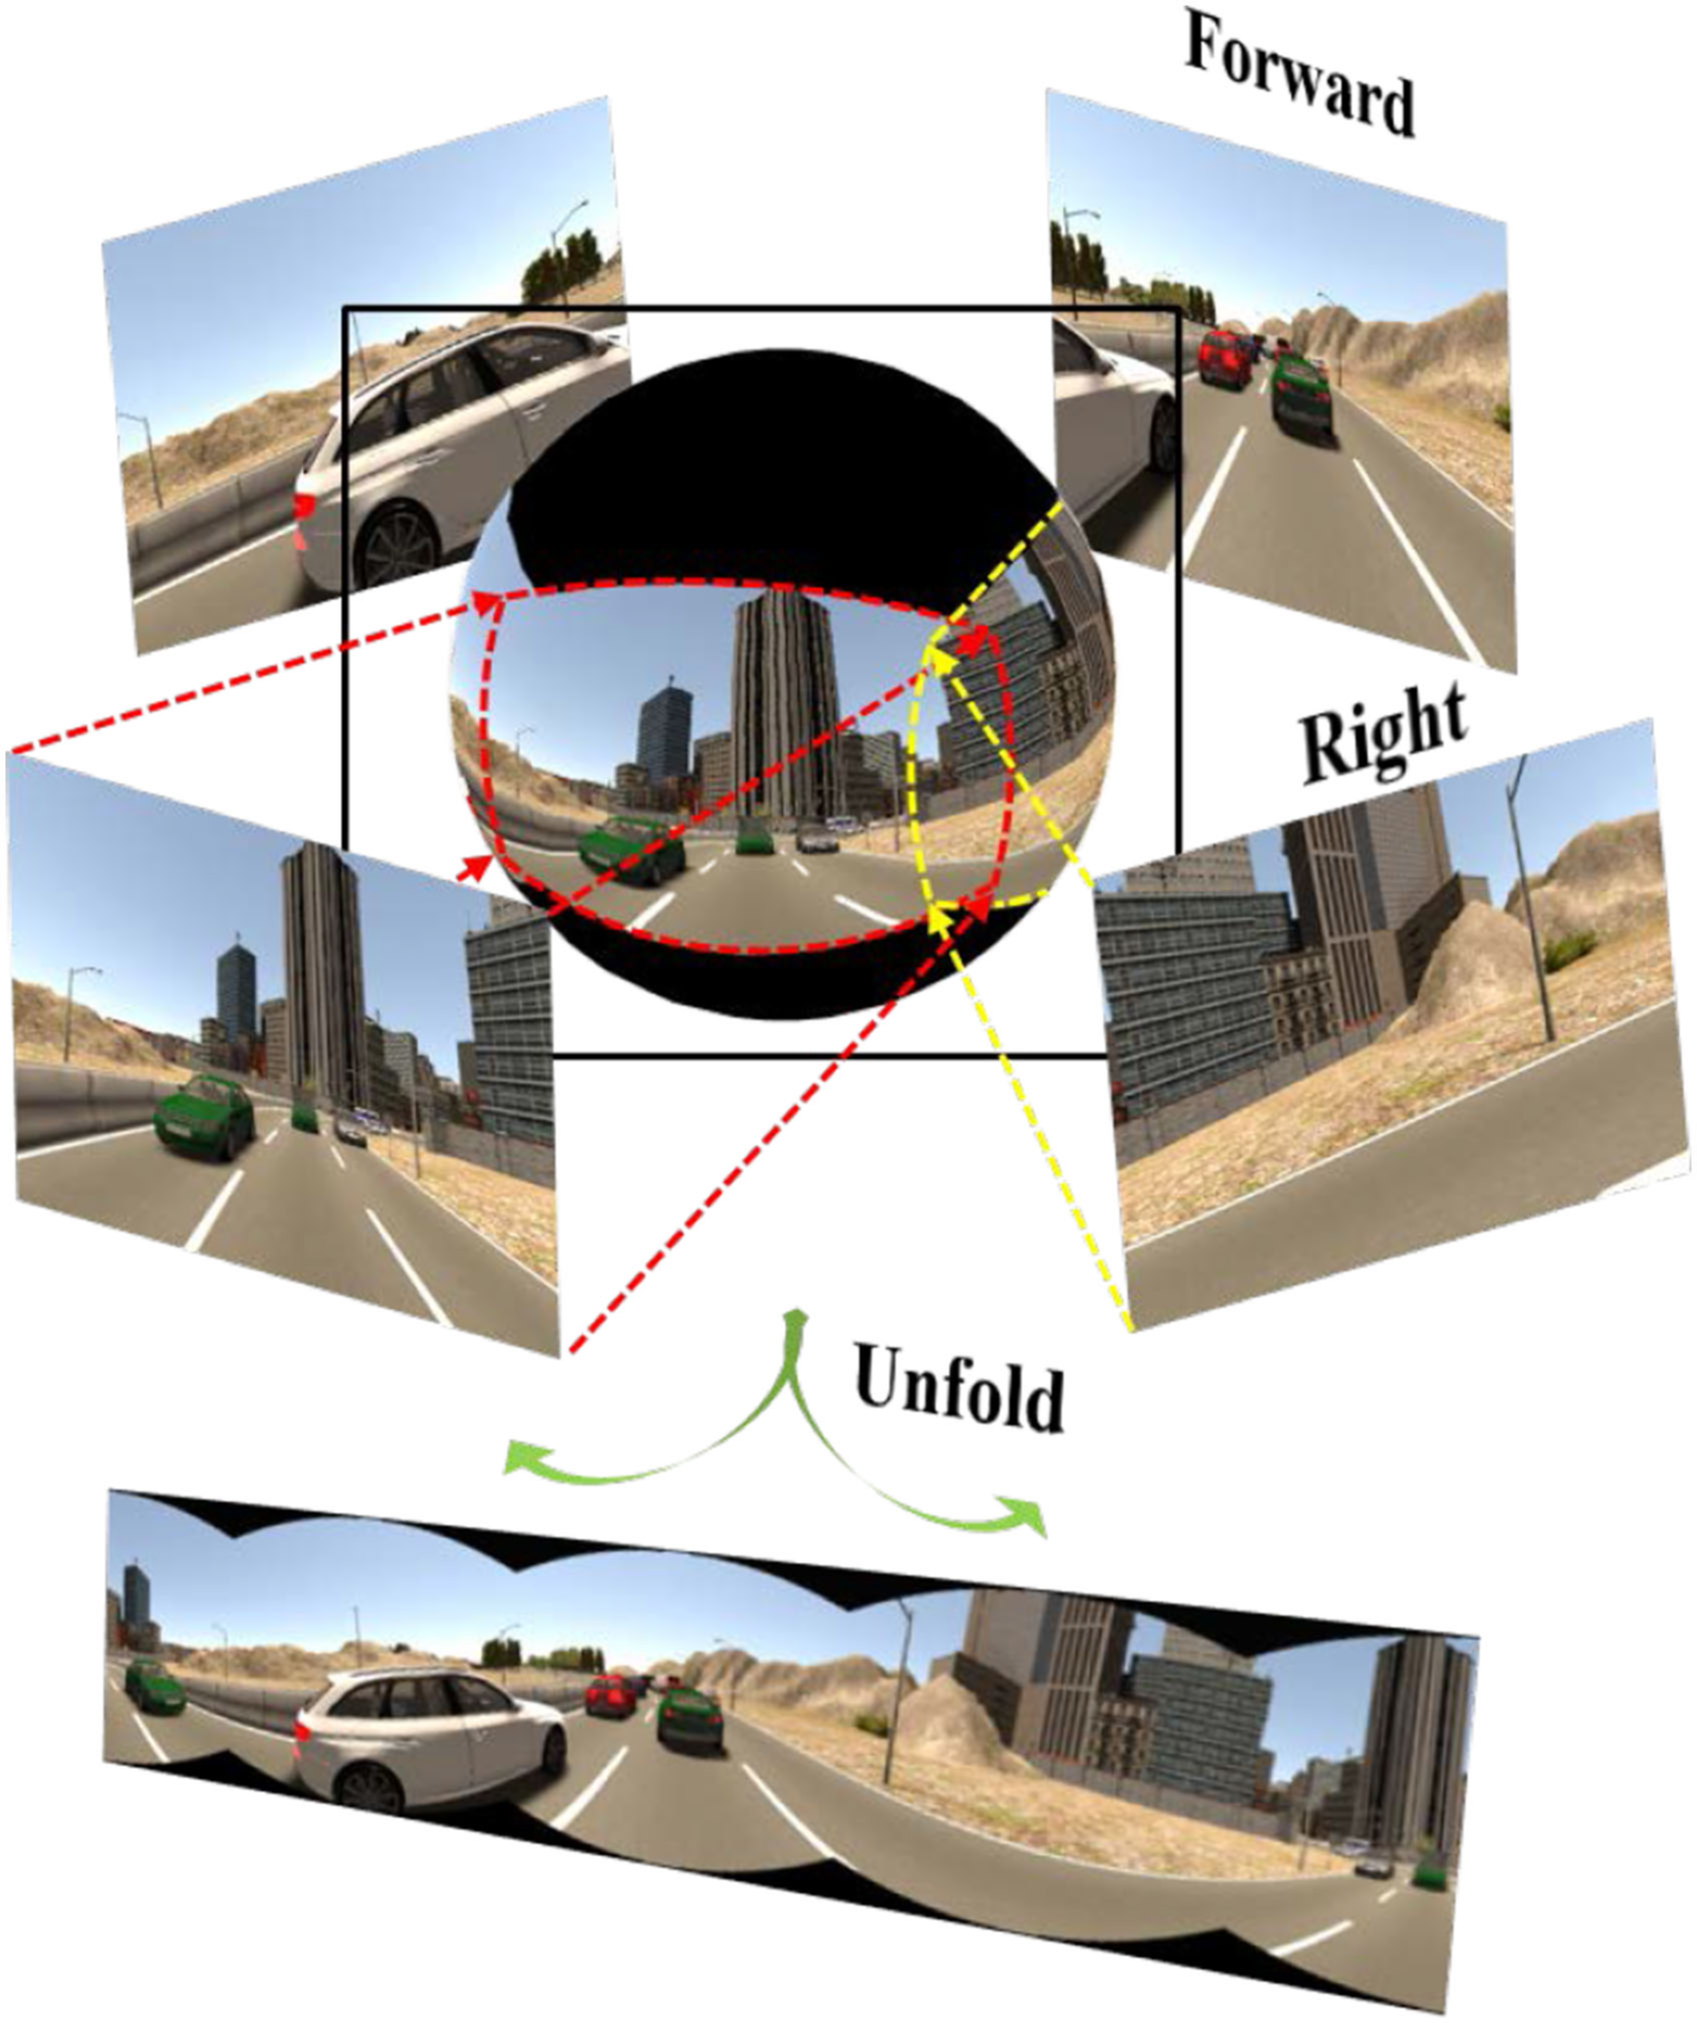
\includegraphics[height=0.7\textheight]{img/duan_esphere}
    \end{figure}
\end{frame}

